\documentclass{article}
\usepackage{graphicx}
\usepackage{hyperref}
\usepackage{geometry}
\usepackage{xcolor}
\usepackage{tcolorbox}
\usepackage{tikz}
\usetikzlibrary{positioning, shapes.geometric, arrows.meta, shadows}
\usepackage{fancyhdr}
\pagestyle{fancy}
\usepackage{pgf-pie} 

\hypersetup{
  colorlinks=true,
  linkcolor=black,
  urlcolor=blue,
  citecolor=black,
  pdfborder={0 0 0}
}

% Page margins
\geometry{margin=1in}

% Define your palette colors
\definecolor{headerColor}{HTML}{D2B48C} % Tan
\definecolor{primaryColor}{HTML}{8B5A2B} % Brownish
\definecolor{backgroundColor}{HTML}{F4E4C1} % Light beige
\definecolor{sectionColor}{HTML}{F9F9F9} % Very light gray
\definecolor{accentColor}{HTML}{FF6F61} % Vibrant coral



% Custom title page with background
\newenvironment{CustomTitlePage}{
  \begin{titlepage}
  \begin{tikzpicture}[remember picture, overlay]
    \shade[left color=orange!20, right color=orange!10]
      (current page.south west) rectangle (current page.north east);
  \end{tikzpicture}
  \vspace*{2cm}
}{
  \end{titlepage}
}

\begin{document}
% ALL content for the first page inside this environment
\begin{CustomTitlePage}
\centering
    % Main Title
    {\Huge \bfseries \color{primaryColor} RebelInuX White Paper} \\[0.5em]
    % Coin's name
    {\large \textit{RebelInuX (REBL)}} \\[0.5em]
    % Author
    {\large \textit{Clément Landormy, Founder of RebelInuX}} \\[0.5em]
    % Date
    {\large \today} \\[2em]
    % Optional: Add a small logo or icon if you like
    % \includegraphics[width=0.2\textwidth]{your-logo.png} \\[2em]
    % Subtle separator line
    \rule{\textwidth}{0.4pt} \\[2em]
    % Main header or subtitle
    {\LARGE \color{black} The Rebellious Meme Coin Inspired by the Spirit of the Dog that Rips the Rules!} \\[3em]
    % Image
    \includegraphics[width=0.4\textwidth]{RebelInuX.jpg} \\[2em]
    % Intro box
    \begin{tcolorbox}[colback=headerColor!15, colframe=headerColor, boxrule=1.5pt, width=0.75\textwidth, arc=4mm]
        \centering
        {\Large \bfseries Introduction} \\[0.5em]
        RebelInuX is more than just a meme coin — it's a movement built on rebellion and community empowerment. Inspired by the fearless Shiba Inu, our project embodies boldness, humor, and decentralization. Join us as we disrupt, entertain, and redefine the future of meme tokens.
    \end{tcolorbox}
\end{CustomTitlePage}


\fancyhf{}
\fancyhead[C]{RebelInuX \textbar\  Join us: \href{https://x.com/RebelInuX}{Twitter} | \href{https://t.me/+bNrP-ozjM501YWVk}{Telegram} | \href{https://discord.gg/3gBzGY6j}{Discord}}
\fancyfoot[C]{\thepage}

% Rest of document starts here
\newpage
\tableofcontents
\newpage

\vspace{0em}
\section[
  \texorpdfstring{\color{primaryColor}Current Tokenomics}{Current Tokenomics}
]{\color{primaryColor}\textbf{Current Tokenomics}}
\begin{tcolorbox}[colback=headerColor!10!white, colframe=headerColor, boxrule=2pt, width=\textwidth, arc=6mm, left=8mm, right=8mm, top=6mm, bottom=6mm]
% Introduction sentence
\textbf{The RebelInuX's tokenomics are designed to promote sustainability, community growth, and project development through transparent and balanced token allocation.}

\subsection[
  \texorpdfstring{\color{primaryColor}Emission Schedule}{Emission Schedule}
]{\color{primaryColor}Emission Schedule}

The total supply of RebelInuX tokens is fixed at \textbf{13 billion (13,000,000,000)} with \textbf{9 decimals}. No inflation or additional minting is planned; any future adjustments will be transparently communicated.

\subsection[
  \texorpdfstring{\color{primaryColor}Token distribution}{Token distribution}
]{\color{primaryColor}Token distribution}

\begin{itemize}
  \item \textbf{Team \& Development (30\%):} Funds support hiring, software development, project management, and ongoing technical improvements.
  \item \textbf{Community \& Marketing (20\%):} Funds enable marketing campaigns, community initiatives, partnerships, and educational content.
  \item \textbf{Liquidity Pool (40\%):} Resources provide liquidity, facilitate trading, and ensure market stability.
  \item \textbf{Reserve (10\%):} Maintained as a contingency for strategic opportunities, emergencies, or future development.
\end{itemize}

\begin{center}
\begin{tikzpicture}
  % Draw the pie chart
  \node (chart) {
    \begin{tikzpicture}
      \pie[
        radius=3,
        color={orange!70, blue!70, green!70, gray!70},
        explode=0.05,
        text=legend,
      ]{
        30/Team \& Development,
        20/Community \& Marketing,
        40/Liquidity Pool,
        10/Reserve
      }
    \end{tikzpicture}
  };

  % Add the title below the pie chart
  \node[below=0.5cm of chart] {\textit{\underline{Distribution of Funds}}};
\end{tikzpicture}
\end{center}
\subsection[
  \texorpdfstring{\color{primaryColor}Token Sale and Allocation Details}{Token Sale and Allocation Details}
]{\color{primaryColor}Token Sale and Allocation Details}
Liquidity will be added via Raydium using a single wallet, while remaining funds are allocated across separate wallets for operations, development, and reserves. Future token distributions will follow the predefined allocations for the team, investors, partners, and ecosystem growth, as detailed in this white paper.
\end{tcolorbox}

\section[
  \texorpdfstring{\color{primaryColor}Future Tokenomics}{Future Tokenomics}
]{\color{primaryColor}\textbf{Future Tokenomics}}
\begin{tcolorbox}[colback=headerColor!10!white, colframe=headerColor, boxrule=2pt, width=\textwidth, arc=6mm, left=8mm, right=8mm, top=6mm, bottom=6mm]
% Introduction sentence
\textbf{RebelInuX's future tokenomics focus on sustainability and community growth through transparent token burns, buy-backs, and vesting strategies, aimed at enhancing token stability and long-term value.}

\subsection[
  \texorpdfstring{\color{primaryColor}Future Burning Mechanism}{Future Burning Mechanism}
]{\color{primaryColor}Future Burning Mechanism}
We are committed to implementing a transparent and systematic token burning process. This mechanism will involve periodically reducing the circulating supply by burning a percentage of tokens from designated wallets. Details such as the \underline{frequency} and \underline{percentage} of tokens to be burned will be communicated clearly through updates on our website and in the white paper.

Stay tuned as we work toward making our ecosystem more \underline{deflationary} and community-driven.

\subsection[
  \texorpdfstring{\color{primaryColor}Vesting and Lock-up Periods}{Vesting and Lock-up Periods}
]{\color{primaryColor}Vesting and Lock-up Periods}
Tokens allocated to the team and advisors will be subject to vesting schedules over a specified period to promote long-term commitment. Additional lock-up periods may also apply to certain allocations to ensure ecosystem stability.

\subsection[
  \texorpdfstring{\color{primaryColor}Token Utility}{Token Utility}
]{\color{primaryColor}Token Utility}
RebelInuX tokens will serve various functions within our ecosystem, including governance voting, staking for rewards, participation in liquidity pools, and potentially, transaction fee discounts.
\subsection[
  \texorpdfstring{\color{primaryColor}Incentives and Rewards}{Incentives and Rewards}
]{\color{primaryColor}Incentives and Rewards}
Participants will earn rewards through staking, liquidity mining, and community activities, aligning incentives to foster ecosystem growth.
\subsection[
  \texorpdfstring{\color{primaryColor}Future Buy-Back Protocol}{Future Buy-Back Protocol}
]{\color{primaryColor}Future Buy-Back Protocol}
In addition to token burns, we plan to implement a \underline{buy-back} mechanism where a portion of the project's revenue or treasury funds will be used to purchase tokens from the open market. This buy-back aims to:

\begin{itemize}
  \item Reduce circulating supply and support token price stability.
  \item Demonstrate ongoing commitment to token value appreciation.
  \item Potentially be complemented by periodic burns of the bought-back tokens.
\end{itemize}

Details such as the \underline{percentage} of revenue allocated for buy-backs, \underline{frequency} of buy-back events, and \underline{mechanics} of execution will be transparently communicated as the protocol is developed.

\end{tcolorbox}

\vspace{1em}


% New Governance Section
\section[
  \texorpdfstring{\color{primaryColor}Governance and Community Participation}{Governance and Community Participation}
]{\color{primaryColor}\textbf{Governance and Community Participation}}

\begin{tcolorbox}[colback=headerColor!10!white, colframe=headerColor, boxrule=2pt, width=\textwidth, arc=6mm, left=8mm, right=8mm, top=6mm, bottom=6mm]
\smallskip
\textbf{\large RebelInuX (REBL)} was initially launched via oriontools.io as a community-oriented meme token, emphasizing fun, engagement, and collective participation. Currently, the token primarily functions as a meme coin, without on-chain governance mechanisms in place.

\subsection[
  \texorpdfstring{\color{primaryColor}Future Governance Framework}{Future Governance Framework}
]{\color{primaryColor}Future Governance Framework}

Recognizing the importance of community involvement in shaping the project's future, the RebelInuX team aims to implement a comprehensive governance system. This will enable token holders to actively participate in key decision-making processes, including proposing initiatives, voting on proposals, and influencing strategic directions—fostering transparency, decentralization, and shared ownership.

\subsection[
  \texorpdfstring{\color{primaryColor}Proposed Governance Protocols}{Proposed Governance Protocols}
]{\color{primaryColor}Proposed Governance Protocols}

The governance system will leverage Solana-compatible protocols such as the Solana Program Library (SPL) Governance or Realms. These platforms will facilitate token staking, proposal submission, and voting, ensuring the community’s voice is central to the project's evolution.

\subsection[
  \texorpdfstring{\color{primaryColor}Community-Driven Development}{Community-Driven Development}
]{\color{primaryColor}Community-Driven Development}

This transition aims to strengthen community trust, promote active engagement, and align project growth with supporter interests. The team is committed to developing an inclusive, secure, and scalable governance model that supports sustainable, community-led decision-making and long-term success.

\smallskip
\end{tcolorbox}

\section[
\texorpdfstring{\color{primaryColor}Decentralization \& Security}{Decentralization \& Security}
]{\color{primaryColor}\textbf{Decentralization \& Security}}
\begin{tcolorbox}[colback=headerColor!10!white, colframe=headerColor, boxrule=2pt, width=\textwidth, arc=6mm, left=8mm, right=8mm, top=6mm, bottom=6mm]

At RebelInuX, our core principles of transparency, decentralization, and security form the foundation of our project. We believe that true empowerment arises from eliminating centralized points of control and fostering a community-driven environment.

To uphold these principles, the project has \textbf{renounced the Freeze Authority, Mint Authority, and Update Authority}. This means:

\begin{itemize}
    \item \textbf{No central authority can freeze or mint new tokens} without community consensus, ensuring fair distribution and safeguarding against malicious actions.
    \item \textbf{All updates and governance decisions are driven by the community}, establishing a trustless and democratic environment.
    \item \textbf{The project operates on Solana’s secure and scalable platform}, leveraging its robust security features to protect our community and assets.
    \item \textbf{Regular audits and transparent reporting} will be conducted to ensure the security and integrity of token allocations and smart contracts.
\end{itemize}

By fully decentralizing our operations, we aim to build an unstoppable rebellion—one resilient to censorship, manipulation, and centralized control. Our commitment to transparency and security is designed to foster trust and ensure that RebelInuX remains a truly community-led movement.

\end{tcolorbox}

\vspace{1em}
\section[
\texorpdfstring{\color{primaryColor}Our Rebellion Roadmap}{Our Rebellion Roadmap}
]{\color{primaryColor}\textbf{Our Rebellion Roadmap}}

\begin{center}
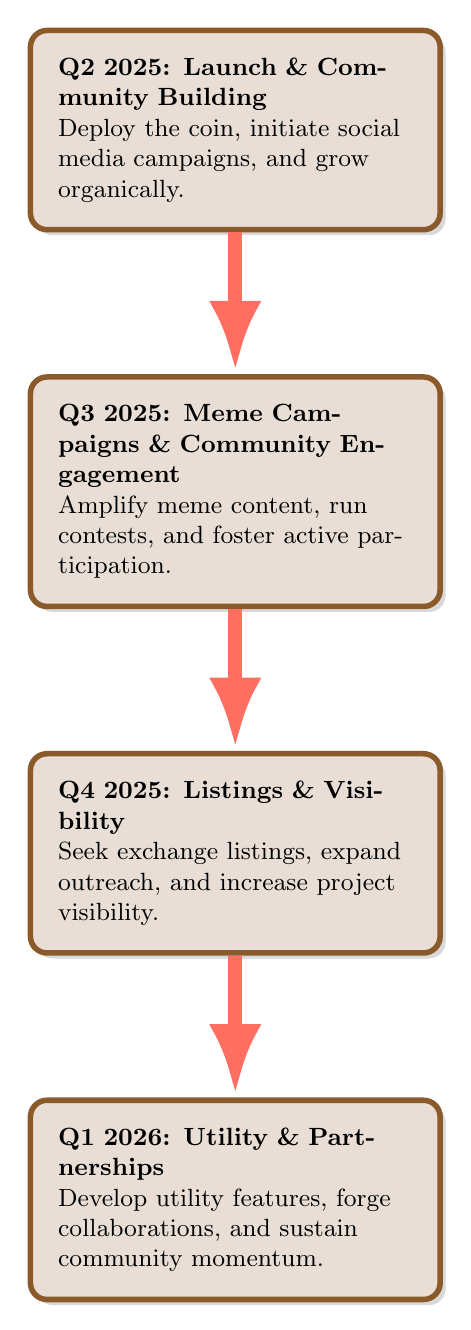
\begin{tikzpicture}[
  node distance=1.8cm and 0cm,
  every node/.style={
    rectangle,
    draw=primaryColor, 
    fill=primaryColor!20, 
    rounded corners=6pt,
    line width=2pt,
    drop shadow={shadow xshift=2pt, shadow yshift=-2pt, opacity=0.3},
    align=left,
    text width=4.5cm,
    inner sep=10pt,
    font=\small
  },
  arrow/.style={
    -Latex,
    thick,
    draw=accentColor,
    shorten >=1pt,
    line width=5pt
  }
]
  % Define nodes
  \node (Q2) {\textbf{Q2 2025: Launch \& Community Building} \\ Deploy the coin, initiate social media campaigns, and grow organically.};
  \node (Q3) [below=of Q2] {\textbf{Q3 2025: Meme Campaigns \& Community Engagement} \\ Amplify meme content, run contests, and foster active participation.};
  \node (Q4) [below=of Q3] {\textbf{Q4 2025: Listings \& Visibility} \\ Seek exchange listings, expand outreach, and increase project visibility.};
  \node (Q1) [below=of Q4] {\textbf{Q1 2026: Utility \& Partnerships} \\ Develop utility features, forge collaborations, and sustain community momentum.};

  % Connect nodes with arrows
  \draw[arrow] (Q2.south) -- (Q3.north);
  \draw[arrow] (Q3.south) -- (Q4.north);
  \draw[arrow] (Q4.south) -- (Q1.north);
\end{tikzpicture}
\end{center}

\vspace{0.5em} % Optional: space between diagram and title

\begin{center}
\textit{\underline{Project Roadmap Timeline}}
\end{center}

\vspace{1em}

% About the Founder with styling
\section[
\texorpdfstring{\color{primaryColor}About the Founder}{About the Founder}
]{\color{primaryColor}\textbf{About the Founder}}

\begin{tcolorbox}[colback=headerColor!10!white, colframe=headerColor, boxrule=0.8mm, width=\textwidth]
\textbf{Clément Landormy} — A dedicated expert in cryptoassets and blockchain technology with over three years of specialized experience gained through his PhD in economics. His expertise encompasses cryptoasset valuation, econometrics, and market analysis.

Clément has conducted extensive empirical research using on-chain data from Binance, Coinbase, and CoinMetrics, focusing on market risks, asset pricing, and financial forecasting. He is proficient in quantitative analysis, financial modeling, programming, and data visualization.

His mission is to develop transparent, innovative, and community-driven blockchain projects that advance the industry and foster trust within the ecosystem.
\end{tcolorbox}

\vspace{1em}

\section[
\texorpdfstring{\color{primaryColor}Meet Our Inspiration: RebelInuX’s Model}{Meet Our Inspiration: RebelInuX’s Model}
]{\color{primaryColor}\textbf{Meet Our Inspiration: RebelInuX’s Model}}
\begin{tcolorbox}[colback=headerColor!10!white, colframe=headerColor, boxrule=0.8mm, width=\textwidth, arc=6mm, left=8mm, right=8mm, top=6mm, bottom=6mm]

\textbf{RebelInuX is more than just a meme coin — it’s a reflection of the loyalty, playfulness, resilience, and strong character embodied by our beloved dog, Idilys.}

\subsection*{About Idilys}

Idilys is a Shiba Inu known for her unwavering loyalty, sharp intelligence, courage, and strong personality. She’s a true rebel at heart — she doesn’t listen much to orders and hates being on a leash. Despite her independence, she’s loving and fiercely loyal. She embodies the spirit of rebellion, community, and perseverance, serving as the perfect symbol of strength and freedom.

\subsection*{Why Idilys?}

Our dog serves as the mascot and inspiration for RebelInuX because:

\begin{itemize}
  \item \textbf{Loyalty}: Like our community, Idilys is fiercely loyal and dedicated.
  \item \textbf{Resilience}: Always bouncing back, just like our token aims to grow and adapt.
  \item \textbf{Independence}: She’s strong-willed and refuses to be controlled — a true reflection of rebellion.
  \item \textbf{Playfulness}: Bringing joy and fun, which is at the heart of our meme culture.
\end{itemize}

\end{tcolorbox}

% Call to Action
\section[
\texorpdfstring{\color{primaryColor}Join the Rebel Pack and Unleash the Rebellion}{Join the Rebel Pack and Unleash the Rebellion}
]{\color{primaryColor}\textbf{Join the Rebel Pack and Unleash the Rebellion}}

We believe in challenging the status quo—fighting injustices in the crypto sphere and beyond. As a community, we stand united in pushing boundaries, standing up for what's right, and making a difference.

We invite our community to share stories, photos, and memories of their dogs, creating a stronger bond and making RebelInuX a truly community-driven project rooted in love, loyalty, and rebellion.

\textit{Together, we are more than just a meme — we are a family that fights for change.}

\vspace{0.5em}

\begin{center}
  \includegraphics[width=0.4\textwidth]{RebelInuX — Unleash the roar - Imgur.jpg}
\end{center}

\vspace{0.5em}

Connect with us on these rebellious platforms and become part of the wildest crypto movement:

\begin{itemize}
  \item \href{https://x.com/RebelInuX}{Twitter}
  \item \href{https://t.me/+bNrP-ozjM501YWVk}{Telegram}
  \item \href{https://discord.gg/3gBzGY6j}{Discord}
\end{itemize}

Join us, share your stories, and help build a vibrant, rebellious community that stands strong together!


\section[
\texorpdfstring{\color{primaryColor}Token Creation and Verification}{Token Creation and Verification}
]{\color{primaryColor}\textbf{Token Creation and Verification}}

\noindent
The \textbf{RebelInuX} token was officially created on \textbf{18 June 2025} at \textbf{20:38 UTC} using \href{https://oriontools.io}{OrionTools.io}, a trusted platform for deploying Solana-based tokens.

\vspace{0.5em}
\noindent
\textbf{Token Address:}
\begin{center}
    \ttfamily \textbf{BfVVGU2an66FVL6qCrx8gJDdgw6EwzmjG672YYD7REmM}
\end{center}

\vspace{0.5em}
\noindent
For transparency and community verification, you can view the token's details, transaction history, and current status on \href{https://solscan.io/token/BfVVGU2an66FVL6qCrx8gJDdgw6EwzmjG672YYD7REmM}{Solscan}.

\bigskip
\noindent
This documentation ensures that the creation process is transparent and verifiable by all community members and stakeholders.

% Legal Disclaimer
\begin{tcolorbox}[colback=backgroundColor!10!white, colframe=headerColor, boxrule=0.8mm, title=Legal Disclaimer, fonttitle=\bfseries]
RebelInuX is a community-driven project designed for entertainment and community engagement. This token is not a security, investment, or financial product and should not be viewed as such. Cryptocurrency investments carry risks, including potential loss of principal. Please conduct your own research and consult with a professional before participating. RebelInuX does not guarantee any financial returns or profits and is not responsible for any damages caused by participation in this project.
\end{tcolorbox}


\vspace{1em}

\begin{center}
\small \textcopyright\, 2025 \\
RebelInuX \quad | \quad \textit{Created by Clément Landormy} \\
All rights reserved.
\end{center}

\end{document}